\documentclass[a4paper,11pt]{article}
\usepackage{amsmath,amsthm,amsfonts,amssymb,amscd,amstext,vmargin,graphics,graphicx,tabularx,multicol} 
\usepackage[francais]{babel}
\usepackage[utf8]{inputenc}  
\usepackage[T1]{fontenc} 
\usepackage{pstricks-add,tikz,tkz-tab,variations}
\usepackage[autolanguage,np]{numprint} 

\setmarginsrb{1.5cm}{0.5cm}{1cm}{0.5cm}{0cm}{0cm}{0cm}{0cm} %Gauche, haut, droite, haut
\newcounter{numexo}
\newcommand{\exo}[1]{\stepcounter{numexo}\noindent{\bf \underline{Exercice~\thenumexo}}}
\reversemarginpar


\newcounter{enumtabi}
\newcounter{enumtaba}
\newcommand{\q}{\stepcounter{enumtabi} \theenumtabi.  }
\newcommand{\qa}{\stepcounter{enumtaba} (\alph{enumtaba}) }
\newcommand{\initq}{\setcounter{enumtabi}{0}}
\newcommand{\initqa}{\setcounter{enumtaba}{0}}

\newcommand{\be}{\begin{enumerate}}
\newcommand{\ee}{\end{enumerate}}
\newcommand{\bi}{\begin{itemize}}
\newcommand{\ei}{\end{itemize}}
\newcommand{\bp}{\begin{pspicture*}}
\newcommand{\ep}{\end{pspicture*}}
\newcommand{\bt}{\begin{tabular}}
\newcommand{\et}{\end{tabular}}
\renewcommand{\tabularxcolumn}[1]{>{\centering}m{#1}} %(colonne m{} centrée, au lieu de p par défault) 
\newcommand{\tnl}{\tabularnewline}

\newcommand{\bmul}[1]{\begin{multicols}{#1}}
\newcommand{\emul}{\end{multicols}}

\newcommand{\trait}{\noindent \rule{\linewidth}{0.2mm}}
\newcommand{\hs}[1]{\hspace{#1}}
\newcommand{\vs}[1]{\vspace{#1}}

\newcommand{\N}{\mathbb{N}}
\newcommand{\Z}{\mathbb{Z}}
\newcommand{\R}{\mathbb{R}}
\newcommand{\C}{\mathbb{C}}
\newcommand{\Dcal}{\mathcal{D}}
\newcommand{\Ccal}{\mathcal{C}}
\newcommand{\mc}{\mathcal}

\newcommand{\vect}[1]{\overrightarrow{#1}}
\newcommand{\ds}{\displaystyle}
\newcommand{\eq}{\quad \Leftrightarrow \quad}
\newcommand{\vecti}{\vec{\imath}}
\newcommand{\vectj}{\vec{\jmath}}
\newcommand{\Oij}{(O;\vec{\imath}, \vec{\jmath})}
\newcommand{\OIJ}{(O;I,J)}




\newcommand{\reponse}[1][1]{%
\multido{}{#1}{\makebox[\linewidth]{\rule[0pt]{0pt}{20pt}\dotfill}
}}

\newcommand{\titre}[5] 
% #1: titre #2: haut gauche #3: bas gauche #4: haut droite #5: bas droite
{
\noindent #2 \hfill #4 \\
#3 \hfill #5

\vspace{-1.6cm}

\begin{center}\rule{6cm}{0.5mm}\end{center}
\vspace{0.2cm}
\begin{center}{\large{\textbf{#1}}}\end{center}
\begin{center}\rule{6cm}{0.5mm}\end{center}
}



\begin{document}
\pagestyle{empty}
\titre{Chapitre 11 : Géométrie dans l'espace et volume}{}{}{}{}

\vspace*{1cm}

\begin{center}
{\Large \textbf{Niveau 1 :}}
\end{center}

\vspace*{1cm}

$\rightarrow$ \textbf{Vocabulaire (sommet, arête, face …)}\\

\vspace*{0.5cm}

\exo \\ Compléter la définition d'un pavé droit.\\

Un pavé droit est un solide composé de six faces . . . . . . . . . . . . . . .\\


\exo \\ Compléter la définition d'une pyramide.\\

Une pyramide est un solide dont :\\
- toutes les faces latérales sont des . . . . . . . . . . . . ayant un sommet commun appelé . . . . . . . . . . . . . de la pyramide,\\
- l'autre face est un polygone quelconque appelé . . . . . . . . . de la pyramide.\\



\exo \\ On considère le parallélépipède ci-dessous. On prend AB = 3 cm et CB = 2 cm.\\
 
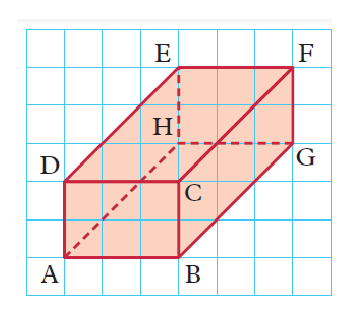
\includegraphics[scale=1]{voca1.eps} \\

\initqa \qa Quelles sont les arrêtes cachées ?\\
\reponse[1]\\

\qa Citer toutes les arrêtes qui mesurent 2 cm.\\
\reponse[1]\\

\exo \\ On considère le parallélépipède ci-dessous. On prend AB = 3 cm et CB = 2 cm.\\
 
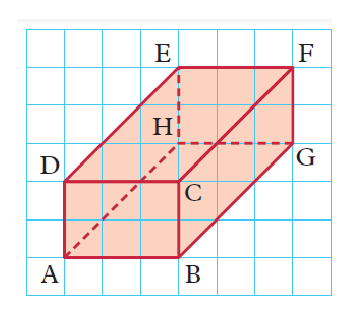
\includegraphics[scale=1]{voca1.eps} \\

\initqa \qa Citer toutes les arrêtes qui mesurent 3 cm.\\
\reponse[1]\\


\qa Citer toutes les arrêtes qui sont égales à CF.\\
\reponse[1]\\


\textbf{Même exercices avec un cube}





\exo \\ On donne le prisme droit à base triangulaire 	ci-dessous. Compléter sa description avec les bons mots de vocabulaire.\\


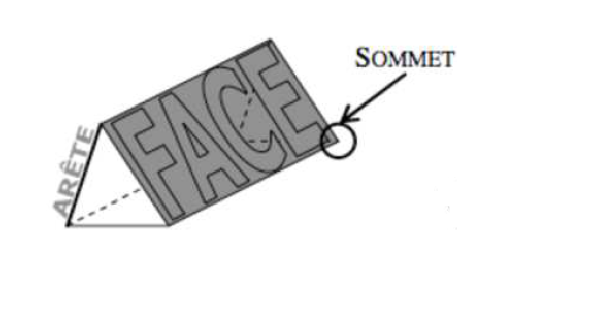
\includegraphics[scale=1]{voca11.eps} \\

Ce prisme droit possède . . . . faces, . . . . arêtes dont . . . . cachées et enfin . . . . sommets.\\

\exo \\ Saurez-vous nommer tous les solides représentés ci-dessous ?\\

\begin{tabular}{|c|c|c|c|}
\hline 
Solide & 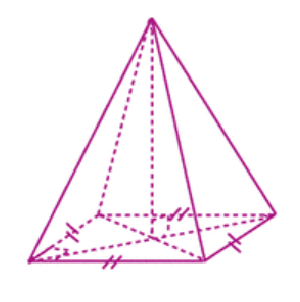
\includegraphics[scale=0.9]{pyramide.eps}  & 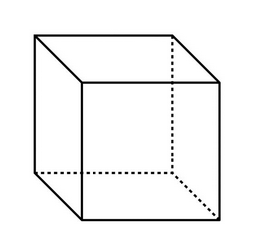
\includegraphics[scale=1]{cube.eps}  & 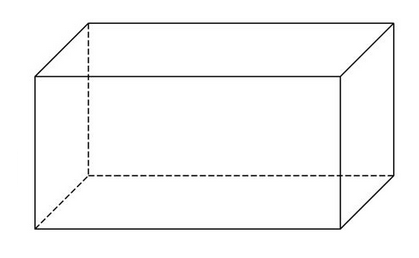
\includegraphics[scale=0.9]{pavedroit.eps}  \\ 
\hline 
Nom du solide & . . . . . . & . . . . . . . & . . . . . . . . \\ 
\hline 
\end{tabular} 

\vspace*{1cm}

$\rightarrow$ \textbf{Conversion de $m^{3}$}\\

\vspace*{0.5cm}


\exo \\ Dans chaque cas, cliquer sur la contenance la plus probable.\\

\begin{tabular}{|c|c|c|c|}
\hline 
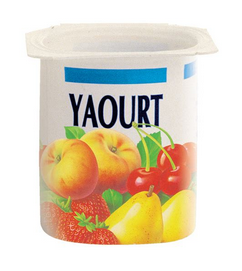
\includegraphics[scale=0.5]{geom1.eps}  & 1 cL & 1 dL  & 1 L \\ 
\hline 
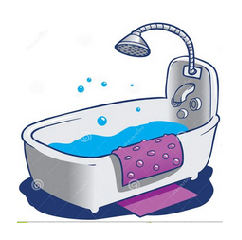
\includegraphics[scale=0.6]{geom2.eps}  & 1 L & 1 daL & 1 hL \\ 
\hline 
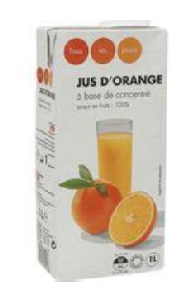
\includegraphics[scale=1=0.3]{geom3.eps}  & 2 L & 2 daL & 2 hL \\ 
\hline 
\end{tabular} 

\vspace*{0.5cm}

\exo \\ 

\renewcommand{\arraystretch}{1.8}

\begin{flushleft}
\begin{tabular}{|p{0,5cm}|p{0,5cm}|p{0,5cm}|p{0,5cm}|p{0,5cm}|p{0,5cm}|p{0,5cm}|p{0,5cm}|p{0,5cm}|p{0,5cm}|p{0,5cm}|p{0,5cm}|p{0,5cm}|p{0,5cm}|p{0,5cm}|p{0,45cm}|p{0,45cm}|p{0,45cm}|p{0,45cm}|p{0,45cm}|p{0,45cm}|}
\hline 
\multicolumn{3}{|c|}{$km^{3}$} & \multicolumn{3}{|c|}{$hm^{3}$} & \multicolumn{3}{|c|}{$dam^{3}$} & \multicolumn{3}{|c|}{$m^{3}$} & \multicolumn{3}{|c|}{$dm^{3}$} & \multicolumn{3}{|c|}{$cm^{3}$} & \multicolumn{3}{|c|}{$mm^{3}$} \\ 
\hline 
 &  &  &  &  &  &  &  &  &  &  &  & hL & daL & L & dL & cL & mL &  &  &  \\ 
\hline 
\end{tabular} 
\end{flushleft}

\vspace*{0.5cm}

On sait que 1 $m^{3}$ = 1 000 $dm^{3}$. Compléter les conversions suivantes en $dm^{3}$.\\

\textbf{Un exemple :} 1,23 $m^{3}$ = 1,23 $\times$ 1 000 $dm^{3}$ = 1 230 $dm^{3}$.\\


\initqa \qa 2,75 $m^{3}$ = . . . . .\\

\qa 0,043 $m^{3}$ = . . . . .\\

\qa 0,91 $m^{3}$ = . . . . .\\








\vspace*{1cm}

$\rightarrow$ \textbf{Calcul de volume}\\

\vspace*{0.5cm}



\exo \\ Écrire la formule permettant de calculer le volume d'un parallélépipède rectangle de longueur L, largeur l et hauteur h.\\


$V = .........................$\\

\exo \\ Écrire la formule permettant de calculer le volume d'un cube  de côté c.\\



$V = .........................$\\





\exo \\ Yann a commencé la construction d'un cube, combien lui manque-t-il de petits cubes pour terminer son solide (un cube de 5 petits cubes de côtés).\\

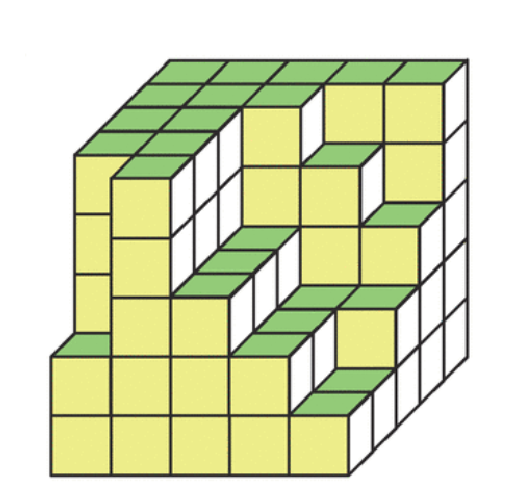
\includegraphics[scale=1]{comptage.eps} \\

Réponse : . . . . .\\


\exo \\ Déterminer le volume de chaque solide en prenant pour unité  le petit cube.\\

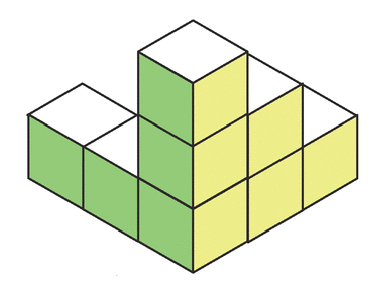
\includegraphics[scale=1]{comptage2.eps} \\

Réponse : . . . . . u.v.\\

\exo \\ Déterminer le volume de chaque solide en prenant pour unité  le petit cube.\\

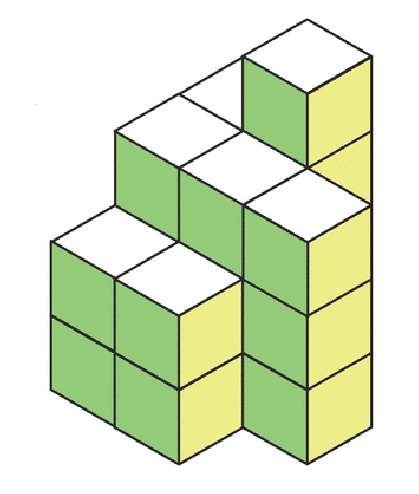
\includegraphics[scale=1]{comptage3.eps} \\

Réponse : . . . . . u.v.\\

\vspace*{0.5cm}

\begin{center}
{\Large \textbf{Niveau 2 :}}
\end{center}

\vspace*{1cm}

$\rightarrow$ \textbf{Vocabulaire (sommet, arête, face …)}\\

\vspace*{0.5cm}



\exo \\ On a représenté ci-dessous le dessin en perspective d'un parallélépipède rectangle.\\
 
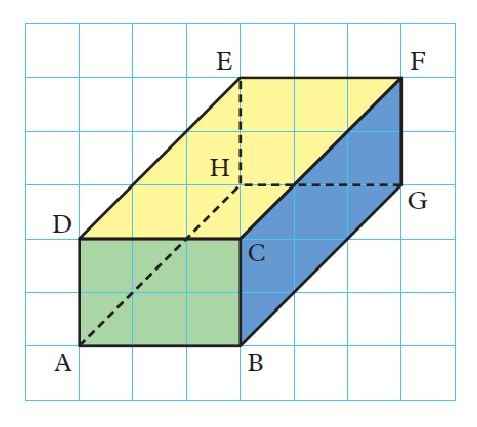
\includegraphics[scale=1]{voca2.eps} \\

\initqa \qa Citer toutes les faces de ce parallélépipède rectangle.\\
\reponse[2]\\


\qa Quelle est la nature de la face ABCD en  réalité ?\\
\reponse[1]\\

\qa Quelle est la nature de la face ABCD sur le dessin ?\\
\reponse[1]\\




\exo \\ On a représenté ci-dessous le dessin en perspective d'un parallélépipède rectangle.\\
 
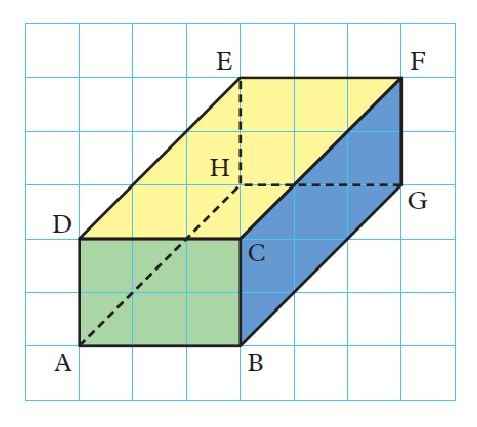
\includegraphics[scale=1]{voca2.eps} \\

\initqa \qa Quelle est la nature de la face BCFG en  réalité ?\\
\reponse[1]\\

\qa Quelle est la nature de la face BCFG sur le dessin ?\\
\reponse[1]\\


\exo \\ On a représenté ci-dessous le dessin en perspective d'un parallélépipède rectangle.\\
 
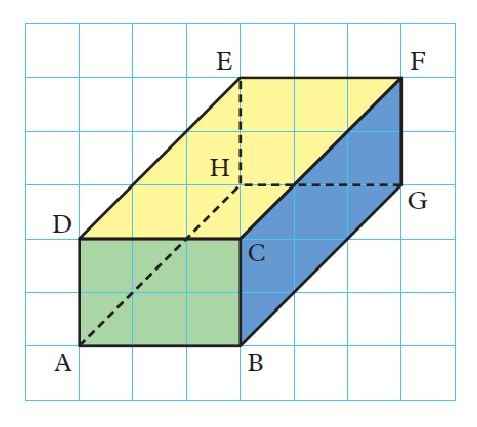
\includegraphics[scale=1]{voca2.eps} \\

\initqa \qa Citer un angle droit en  réalité  et sur le dessin?\\
\reponse[1]\\

\qa Citer un angle droit en réalité mais pas sur le dessin ?\\
\reponse[1]\\

\textbf{Même exercices avec un cube}\\

\exo \\ On donne la pyramide ci-dessous. Compléter sa description avec les bons mots de vocabulaire.\\



\includegraphics[scale=1]{voca12.eps} \\

Cette pyramide possède . . . . faces, . . . . arêtes dont . . . . cachées et enfin . . . . sommets.\\



\exo \\ Saurez-vous nommer tous les solides représentés ci-dessous ?\\

\begin{tabular}{|c|c|c|c|}
\hline 
Solide &  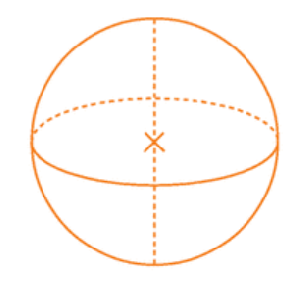
\includegraphics[scale=1]{sphere.eps}  & 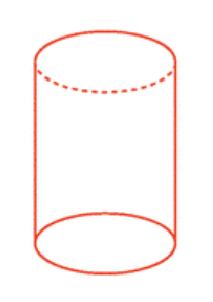
\includegraphics[scale=1]{cylindre.eps}   & 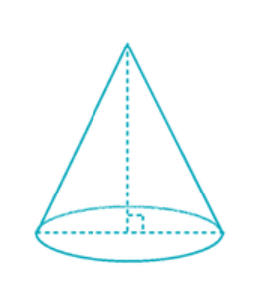
\includegraphics[scale=1]{cone.eps}   \\ 
\hline 
Nom du solide & . . . . . . & . . . . . . . & . . . . . . . . \\ 
\hline 
\end{tabular} 

\vspace*{0.5cm}


\vspace*{1cm}

$\rightarrow$ \textbf{Conversion de $m^{3}$}\\

\vspace*{0.5cm}



\exo \\

\renewcommand{\arraystretch}{1.8}

\begin{flushleft}
\begin{tabular}{|p{0,5cm}|p{0,5cm}|p{0,5cm}|p{0,5cm}|p{0,5cm}|p{0,5cm}|p{0,5cm}|p{0,5cm}|p{0,5cm}|p{0,5cm}|p{0,5cm}|p{0,5cm}|p{0,5cm}|p{0,5cm}|p{0,5cm}|p{0,45cm}|p{0,45cm}|p{0,45cm}|p{0,45cm}|p{0,45cm}|p{0,45cm}|}
\hline 
\multicolumn{3}{|c|}{$km^{3}$} & \multicolumn{3}{|c|}{$hm^{3}$} & \multicolumn{3}{|c|}{$dam^{3}$} & \multicolumn{3}{|c|}{$m^{3}$} & \multicolumn{3}{|c|}{$dm^{3}$} & \multicolumn{3}{|c|}{$cm^{3}$} & \multicolumn{3}{|c|}{$mm^{3}$} \\ 
\hline 
 &  &  &  &  &  &  &  &  &  &  &  & hL & daL & L & dL & cL & mL &  &  &  \\ 
\hline 
\end{tabular} 
\end{flushleft}

\vspace*{0.5cm}

 On sait que 1 $mm^{3}$ = 0,001 $cm^{3}$. Compléter les conversions suivantes en $cm^{3}$.\\
\textbf{Un exemple :} 134 $mm^{3}$ = 134 $\times$ 0,001 $cm^{3}$ = 0,134 $cm^{3}$.\\


\initqa \qa 227 $mm^{3}$ = . . . . .\\

\qa 3 916 $mm^{3}$ = . . . . .\\

\qa 55,4 $mm^{3}$ = . . . . .\\

\exo \\ 

\renewcommand{\arraystretch}{1.8}

\begin{flushleft}
\begin{tabular}{|p{0,5cm}|p{0,5cm}|p{0,5cm}|p{0,5cm}|p{0,5cm}|p{0,5cm}|p{0,5cm}|p{0,5cm}|p{0,5cm}|p{0,5cm}|p{0,5cm}|p{0,5cm}|p{0,5cm}|p{0,5cm}|p{0,5cm}|p{0,45cm}|p{0,45cm}|p{0,45cm}|p{0,45cm}|p{0,45cm}|p{0,45cm}|}
\hline 
\multicolumn{3}{|c|}{$km^{3}$} & \multicolumn{3}{|c|}{$hm^{3}$} & \multicolumn{3}{|c|}{$dam^{3}$} & \multicolumn{3}{|c|}{$m^{3}$} & \multicolumn{3}{|c|}{$dm^{3}$} & \multicolumn{3}{|c|}{$cm^{3}$} & \multicolumn{3}{|c|}{$mm^{3}$} \\ 
\hline 
 &  &  &  &  &  &  &  &  &  &  &  & hL & daL & L & dL & cL & mL &  &  &  \\ 
\hline 
\end{tabular} 
\end{flushleft}

\vspace*{0.5cm}

Convertir dans l'unité demandée.\\

\initqa \qa 1 L = .......... cl\\

\qa 23,5 mL = .......... cL\\
 
 
\qa 5,324 daL = .......... dL \\

\qa 176,2 dL  = ........... hL\\



\exo \\ 

\renewcommand{\arraystretch}{1.8}

\begin{flushleft}
\begin{tabular}{|p{0,5cm}|p{0,5cm}|p{0,5cm}|p{0,5cm}|p{0,5cm}|p{0,5cm}|p{0,5cm}|p{0,5cm}|p{0,5cm}|p{0,5cm}|p{0,5cm}|p{0,5cm}|p{0,5cm}|p{0,5cm}|p{0,5cm}|p{0,45cm}|p{0,45cm}|p{0,45cm}|p{0,45cm}|p{0,45cm}|p{0,45cm}|}
\hline 
\multicolumn{3}{|c|}{$km^{3}$} & \multicolumn{3}{|c|}{$hm^{3}$} & \multicolumn{3}{|c|}{$dam^{3}$} & \multicolumn{3}{|c|}{$m^{3}$} & \multicolumn{3}{|c|}{$dm^{3}$} & \multicolumn{3}{|c|}{$cm^{3}$} & \multicolumn{3}{|c|}{$mm^{3}$} \\ 
\hline 
 &  &  &  &  &  &  &  &  &  &  &  & hL & daL & L & dL & cL & mL &  &  &  \\ 
\hline 
\end{tabular} 
\end{flushleft}

\vspace*{0.5cm}

Compléter avec la bonne unité de capacité.\\


\initqa \qa 200 L = 2 . . .\\

\qa 0,065 hL = 65 . . .\\

\qa 87 000 mL = 8,7 . . .\\

\qa 4,01 mL = 0,401 . . .\\

\qa 3 205 daL = 32,05 . . .\\



\vspace*{1cm}

$\rightarrow$ \textbf{Calcul de volume}\\

\vspace*{0.5cm}





\exo \\ Compléter le tableau suivant, l'objectif est de trouver le volume des 2 solides donnés.\\

\begin{tabular}{|c|c|c|c|c|}
\hline 
 & Longueur & Largeur & Hauteur & Volume du solide \\ 
\hline 
Solide 1 & 6 cm & 5 cm & 4 cm & . . . . \\ 
\hline 
Solide 2 & 8 m & 1 m & 2 m & . . . . \\ 
\hline 
\end{tabular} 



\exo \\ Calculer le volume d'un cube de côté 5 cm.\\

Formule : . . . . . . . . . . . . . . . . . . .\\

Calculs : . . . . . . . . . . . . . . . . . . .\\

Réponse : . . . . . . . . . . . . . . . . . . .\\


\exo \\ Calculer le volume d'un parallélépipède rectangle de longueur 10 cm, de largeur 8,5 cm de hauteur 2 cm.\\

Formule : . . . . . . . . . . . . . . . . . . .\\

Calculs : . . . . . . . . . . . . . . . . . . .\\

Réponse : . . . . . . . . . . . . . . . . . . .\\


\exo \\ Calculer le volume du solide suivant.\\

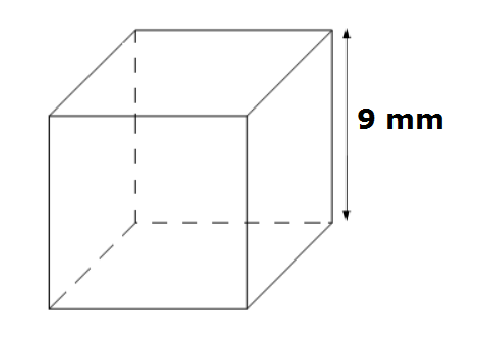
\includegraphics[scale=1]{cube2.eps} \\

Formule : . . . . . . . . . . . . . . . . . . .\\

Calculs : . . . . . . . . . . . . . . . . . . .\\

Réponse : . . . . . . . . . . . . . . . . . . .\\



\exo \\ Calculer le volume du solide suivant.\\

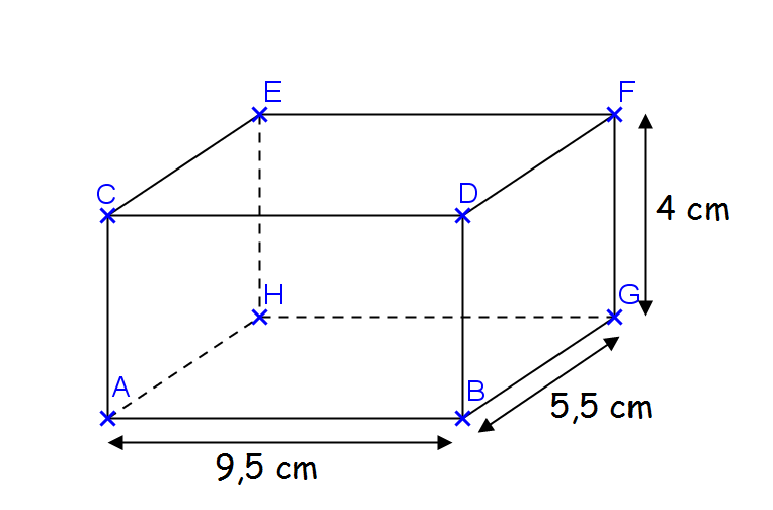
\includegraphics[scale=1]{pavedroit2.eps} \\

Formule : . . . . . . . . . . . . . . . . . . .\\

Calculs : . . . . . . . . . . . . . . . . . . .\\

Réponse : . . . . . . . . . . . . . . . . . . .\\







\begin{center}
{\Large \textbf{Niveau 3 :}}
\end{center}

\vspace*{1cm}

$\rightarrow$ \textbf{Vocabulaire (sommet, arête, face …)}\\

\vspace*{0.5cm}

\exo \\ On donne le prisme droit à base hexagonale ci-dessous. Compléter sa description avec les bons mots de vocabulaire.\\


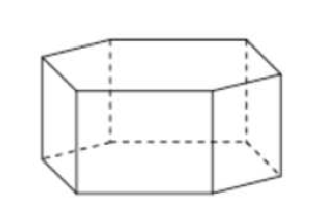
\includegraphics[scale=1]{voca13.eps} \\

Ce prisme droit possède . . . . faces, . . . . arêtes dont . . . . cachées et enfin . . . . sommets.\\


\exo \\ On considère la figure ci-dessous.\\
 
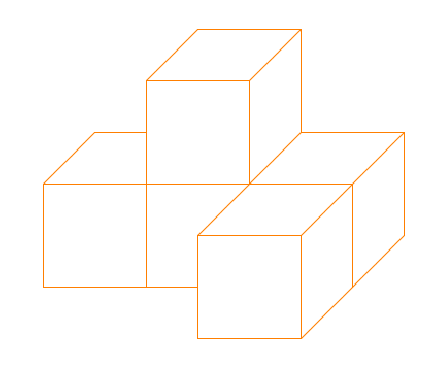
\includegraphics[scale=1]{voca3.eps} \\

Combien y a-t-il de cube dans cette figure ?\\

Réponse : . . . . . . . . . . . . . \\


\exo \\ Voici le patron d'un cube : \\

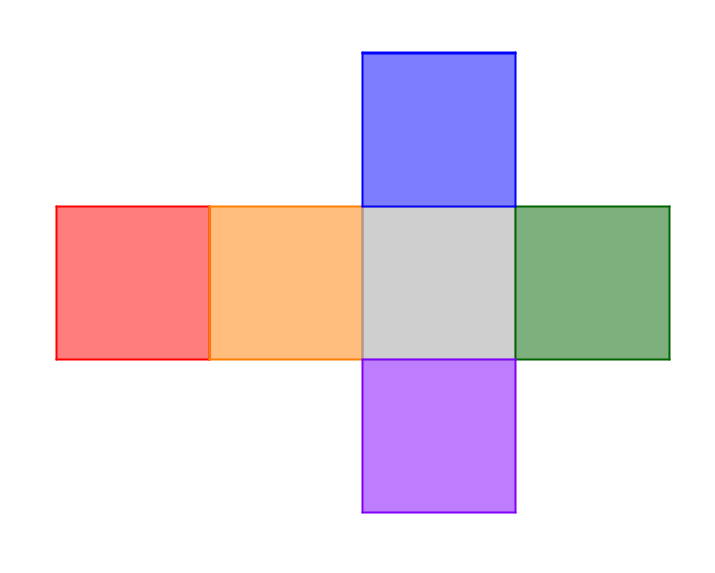
\includegraphics[scale=1]{voca4.eps} \\

Lorsque l'on forme le cube, quelle est la couleur de la face supérieure s'il est posé sur la face rouge ?\\
\reponse[1]\\

\exo \\ Voici le patron d'un cube : \\

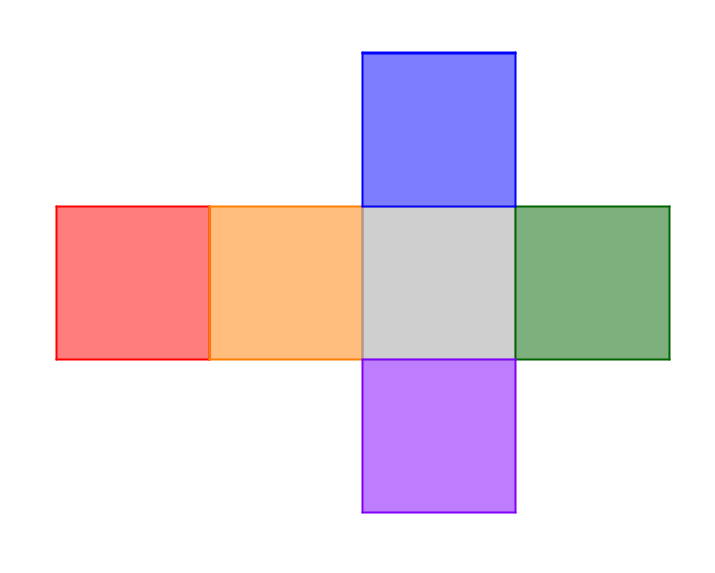
\includegraphics[scale=1]{voca4.eps} \\

Lorsque l'on forme le cube, quelle est la couleur de la face supérieure s'il est posé sur la face violette ?\\
\reponse[1]\\


\exo \\ Voici le patron d'un cube : \\

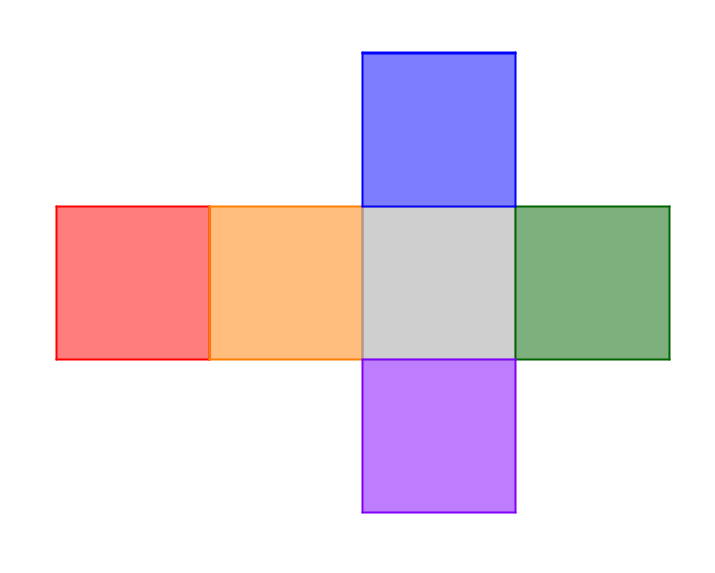
\includegraphics[scale=1]{voca4.eps} \\

Lorsque l'on forme le cube, quelle est la couleur de la face supérieure s'il est posé sur la face bleue ?\\
\reponse[1]\\


\textbf{Pour plus tard} : cube à terminé.\\
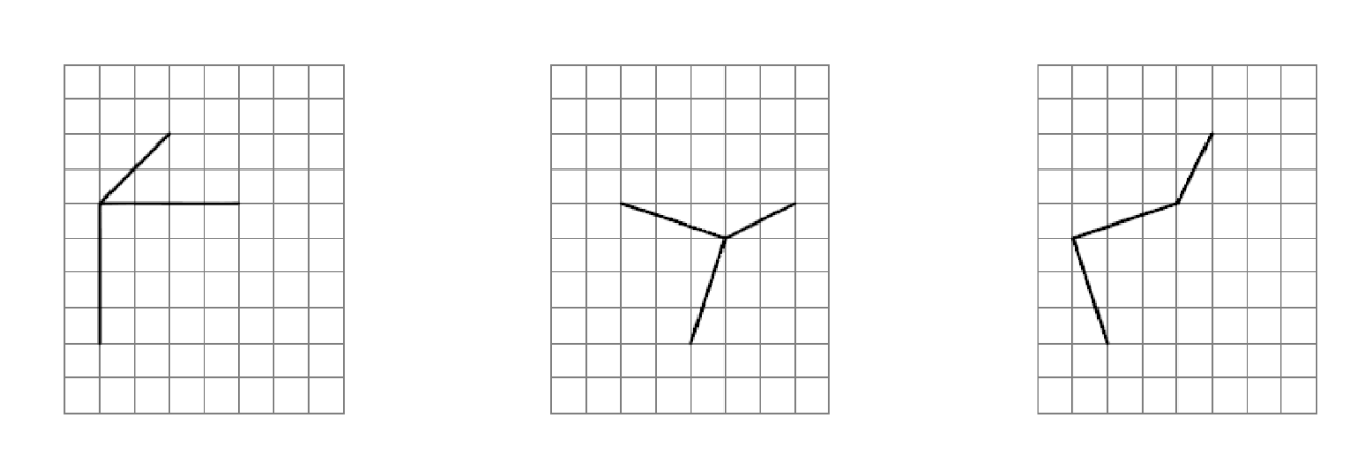
\includegraphics[scale=0.8]{voca14.eps} \\


\exo \\ Saurez-vous nommer tous les solides représentés ci-dessous ?\\

\begin{tabular}{|c|c|c|c|}
\hline 
Solide &  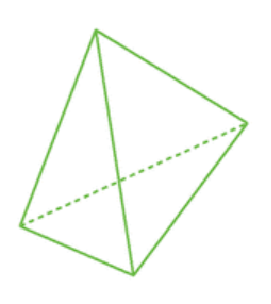
\includegraphics[scale=1]{pyramide2.eps}  & 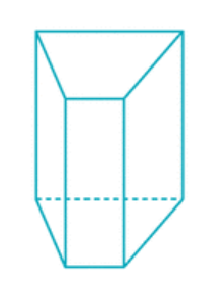
\includegraphics[scale=1]{prismedroit.eps}   & 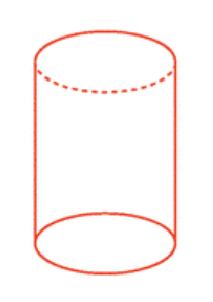
\includegraphics[scale=1]{cylindre.eps}   \\ 
\hline 
Nom du solide & . . . . . . & . . . . . . . & . . . . . . . . \\ 
\hline 
\end{tabular} 

\vspace*{0.5cm}


\vspace*{1cm}

$\rightarrow$ \textbf{Conversion de $m^{3}$}\\

\vspace*{0.5cm}



\exo \\

\renewcommand{\arraystretch}{1.8}

\begin{flushleft}
\begin{tabular}{|p{0,5cm}|p{0,5cm}|p{0,5cm}|p{0,5cm}|p{0,5cm}|p{0,5cm}|p{0,5cm}|p{0,5cm}|p{0,5cm}|p{0,5cm}|p{0,5cm}|p{0,5cm}|p{0,5cm}|p{0,5cm}|p{0,5cm}|p{0,45cm}|p{0,45cm}|p{0,45cm}|p{0,45cm}|p{0,45cm}|p{0,45cm}|}
\hline 
\multicolumn{3}{|c|}{$km^{3}$} & \multicolumn{3}{|c|}{$hm^{3}$} & \multicolumn{3}{|c|}{$dam^{3}$} & \multicolumn{3}{|c|}{$m^{3}$} & \multicolumn{3}{|c|}{$dm^{3}$} & \multicolumn{3}{|c|}{$cm^{3}$} & \multicolumn{3}{|c|}{$mm^{3}$} \\ 
\hline 
 &  &  &  &  &  &  &  &  &  &  &  & hL & daL & L & dL & cL & mL &  &  &  \\ 
\hline 
\end{tabular} 
\end{flushleft}

\vspace*{0.5cm}

 On sait que 1 $dm^{3}$ = 1 L. Convertir d'abord toutes les valeurs en $dm^{3}$ puis donner leur valeur en L.\\

\initqa \qa 25,36 $m^{3}$ = . . . . . $dm^{3}$ = . . . . . . L\\

\qa 13 500 $cm^{3}$ = . . . . . $dm^{3}$ = . . . . . . L\\


\qa 0,108 $dam^{3}$ = . . . . . $dm^{3}$ = . . . . . . L\\



\exo \\ 

\renewcommand{\arraystretch}{1.8}

\begin{flushleft}
\begin{tabular}{|p{0,5cm}|p{0,5cm}|p{0,5cm}|p{0,5cm}|p{0,5cm}|p{0,5cm}|p{0,5cm}|p{0,5cm}|p{0,5cm}|p{0,5cm}|p{0,5cm}|p{0,5cm}|p{0,5cm}|p{0,5cm}|p{0,5cm}|p{0,45cm}|p{0,45cm}|p{0,45cm}|p{0,45cm}|p{0,45cm}|p{0,45cm}|}
\hline 
\multicolumn{3}{|c|}{$km^{3}$} & \multicolumn{3}{|c|}{$hm^{3}$} & \multicolumn{3}{|c|}{$dam^{3}$} & \multicolumn{3}{|c|}{$m^{3}$} & \multicolumn{3}{|c|}{$dm^{3}$} & \multicolumn{3}{|c|}{$cm^{3}$} & \multicolumn{3}{|c|}{$mm^{3}$} \\ 
\hline 
 &  &  &  &  &  &  &  &  &  &  &  & hL & daL & L & dL & cL & mL &  &  &  \\ 
\hline 
\end{tabular} 
\end{flushleft}

\vspace*{0.5cm}

Convertir dans l'unité demandée.\\

\initqa \qa 1 $m^{3}$ = . . . . $dm^{3}$.\\

\qa 1 $dam^{3}$ = . . . . $m^{3}$.\\

\qa 1 $dm^{3}$ = . . . . $m^{3}$.\\

\qa 1 $m^{3}$ = . . . . $dam^{3}$.\\

\qa 1 L = . . . . $cm^{3}$.\\

\qa  1 mL = . . . . $cm^{3}$.\\








\vspace*{1cm}

$\rightarrow$ \textbf{Calcul de volume}\\

\vspace*{0.5cm}


\exo \\ La piscine de mes amis est rectangulaire. Elle mesure 9,8 m sur 8,7 m et elle a une profondeur de 1,2 m.\\

Cliquer sur la bonne réponse.\\

\begin{tabular}{|c|c|c|c|c|}
\hline 
Son volume est proche de ... & 1 $m^{3}$ & 10 $m^{3}$ & 100 $m^{3}$ & 1 000 $m^{3}$ \\ 
\hline 
La quantité d'eau nécessaire a la remplir est proche de ... & 1 L & 1 000 L & 10 000 L & 100 000 L \\ 
\hline 
\end{tabular} 


\exo \\ Compléter le tableau suivant, l'objectif est de trouver le volume des 2 solides donnés.\\

\begin{tabular}{|c|c|c|c|c|}
\hline 
 & Longueur & Largeur & Hauteur & Volume du solide \\ 
\hline 
Solide 1 & 2 m & 4,5 dm & 6 dm & . . . . \\ 
\hline 
Solide 2 & 96 mm & 7,5 cm & 0,45 dm & . . . . \\ 
\hline 
\end{tabular} 



\exo \\ Calculer le volume du solide suivant.\\

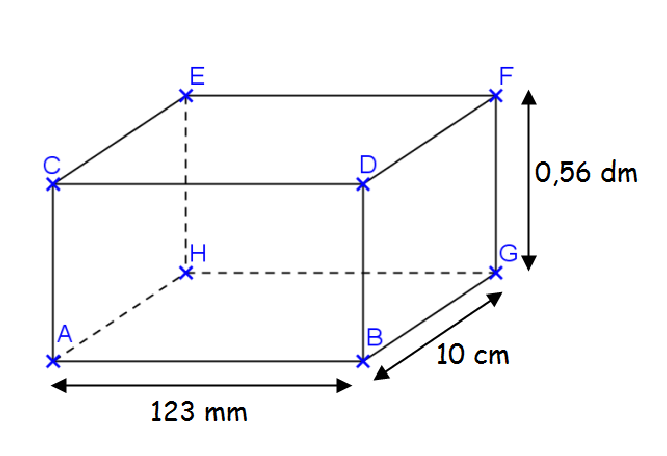
\includegraphics[scale=1]{vol1.eps} \\

Formule : . . . . . . . . . . . . . . . . . . .\\

Calculs : . . . . . . . . . . . . . . . . . . .\\

Réponse : . . . . . . . . . . . . . . . . . . .\\




\begin{center}
{\Large \textbf{Niveau 4:}}
\end{center}

\vspace*{1cm}

$\rightarrow$ \textbf{Vocabulaire (sommet, arête, face …)}\\

\vspace*{0.5cm}

\exo \\ Parmi ces 6 figures, citer celles qui correspondent au patron d'un cube.\\



\begin{flushleft}
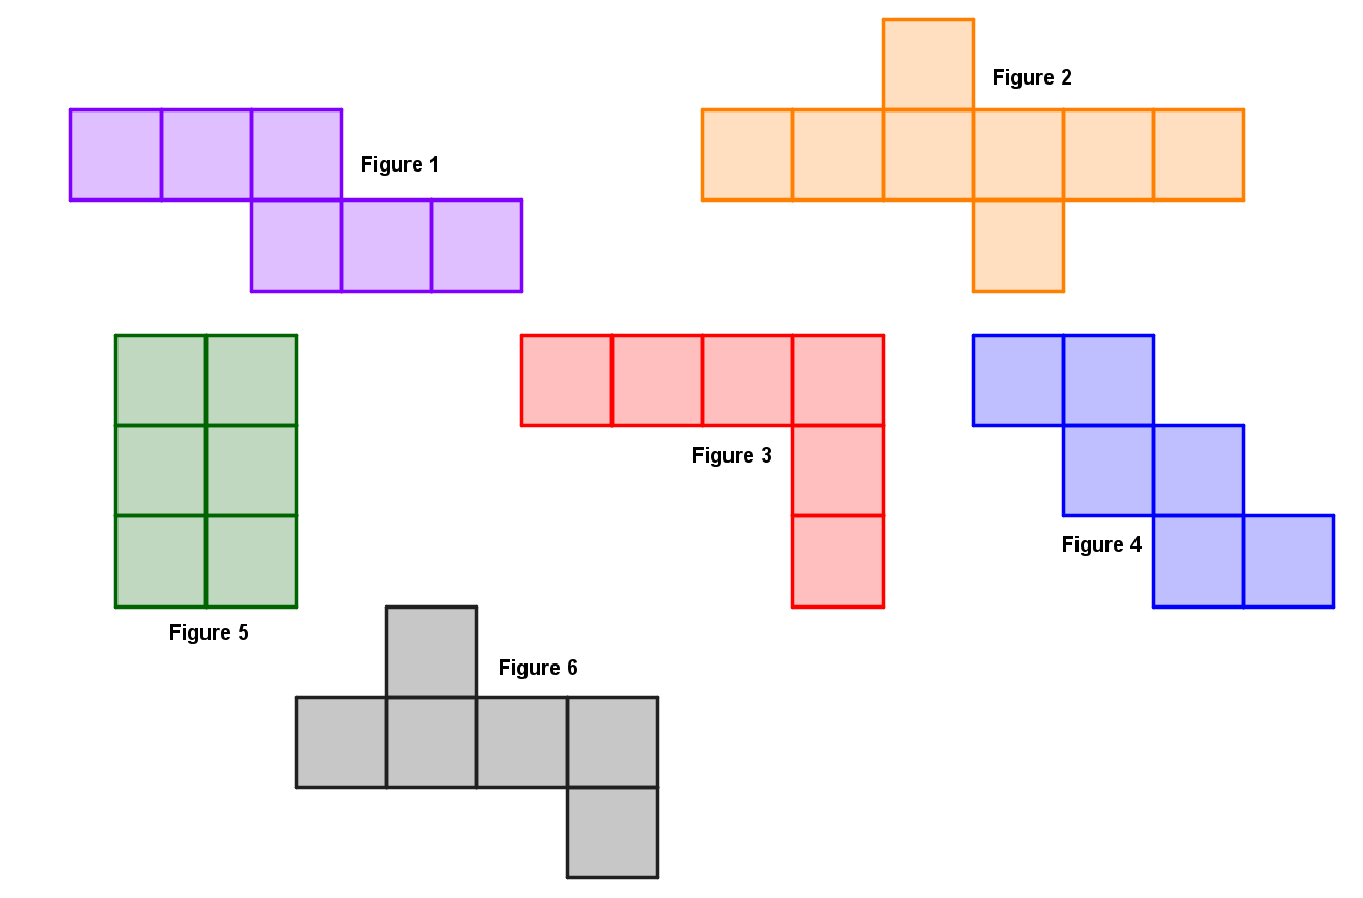
\includegraphics[scale=0.85]{voca5.eps} 
\end{flushleft}\reponse[1]\\


\exo \\ Lorsque l'on observe un dé à jouer classique, si on lit "2" sur la face supérieure, on aura un "5" sur la face inférieure.
De même, si on lit un "3" sur la face supérieure, on aura un "4" sur la face inférieure.\\

\initqa
\qa Que vaut alors la somme des points de deux faces opposées ?\\
\reponse[1]\\


\qa Chacun des deux patrons ci-dessous peut-il être celui de votre dé ?\\

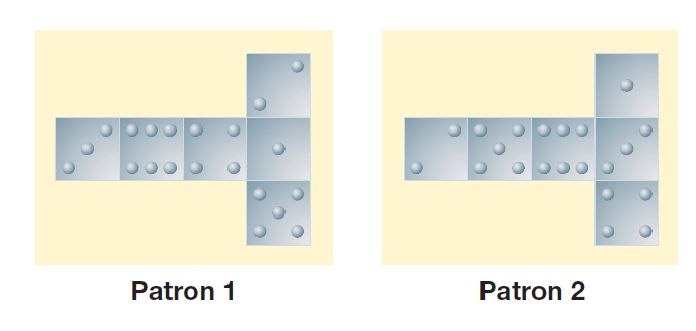
\includegraphics[scale=1]{voca7.eps} \\
\reponse[1]\\

\vspace*{1cm}

$\rightarrow$ \textbf{Conversion de $m^{3}$}\\

\vspace*{0.5cm}


\exo \\ 

\renewcommand{\arraystretch}{1.8}

\begin{flushleft}
\begin{tabular}{|p{0,5cm}|p{0,5cm}|p{0,5cm}|p{0,5cm}|p{0,5cm}|p{0,5cm}|p{0,5cm}|p{0,5cm}|p{0,5cm}|p{0,5cm}|p{0,5cm}|p{0,5cm}|p{0,5cm}|p{0,5cm}|p{0,5cm}|p{0,45cm}|p{0,45cm}|p{0,45cm}|p{0,45cm}|p{0,45cm}|p{0,45cm}|}
\hline 
\multicolumn{3}{|c|}{$km^{3}$} & \multicolumn{3}{|c|}{$hm^{3}$} & \multicolumn{3}{|c|}{$dam^{3}$} & \multicolumn{3}{|c|}{$m^{3}$} & \multicolumn{3}{|c|}{$dm^{3}$} & \multicolumn{3}{|c|}{$cm^{3}$} & \multicolumn{3}{|c|}{$mm^{3}$} \\ 
\hline 
 &  &  &  &  &  &  &  &  &  &  &  & hL & daL & L & dL & cL & mL &  &  &  \\ 
\hline 
\end{tabular} 
\end{flushleft}

\vspace*{0.5cm}

Convertir dans l'unité demandée.\\

\initqa \qa 200 $mm^{3}$ = . . . . . $cm^{3}$.\\

\qa 6 023 $km^{3}$ = . . . . . $dam^{3}$.\\

\qa 47,365 $cm^{3}$ = . . . . . $mm^{3}$.\\

\qa 900 514 $m^{3}$ = . . . . . $km^{3}$.\\

\qa 1 mL = . . . . . $cm^{3}$.\\

\qa 0,72 hl = . . . . . $m^{3}$.\\


\exo \\ 

\renewcommand{\arraystretch}{1.8}

\begin{flushleft}
\begin{tabular}{|p{0,5cm}|p{0,5cm}|p{0,5cm}|p{0,5cm}|p{0,5cm}|p{0,5cm}|p{0,5cm}|p{0,5cm}|p{0,5cm}|p{0,5cm}|p{0,5cm}|p{0,5cm}|p{0,5cm}|p{0,5cm}|p{0,5cm}|p{0,45cm}|p{0,45cm}|p{0,45cm}|p{0,45cm}|p{0,45cm}|p{0,45cm}|}
\hline 
\multicolumn{3}{|c|}{$km^{3}$} & \multicolumn{3}{|c|}{$hm^{3}$} & \multicolumn{3}{|c|}{$dam^{3}$} & \multicolumn{3}{|c|}{$m^{3}$} & \multicolumn{3}{|c|}{$dm^{3}$} & \multicolumn{3}{|c|}{$cm^{3}$} & \multicolumn{3}{|c|}{$mm^{3}$} \\ 
\hline 
 &  &  &  &  &  &  &  &  &  &  &  & hL & daL & L & dL & cL & mL &  &  &  \\ 
\hline 
\end{tabular} 
\end{flushleft}

\vspace*{0.5cm}

Compléter avec la bonne unité.\\

\initqa \qa 1 000 000 $cm^{3}$ = 0,000 001 . . . \\

 \qa 2 541  $mm^{3}$ = 0,000 002 541 . . . \\
 
  \qa 33 $dam^{3}$ =  33 000 000 . . . \\
  
   \qa 0 005 63 $cm^{3}$ = 5 630 . . . \\




\vspace*{1cm}

$\rightarrow$ \textbf{Calcul de volume}\\

\vspace*{0.5cm}




\exo \\ Compléter le tableau suivant, l'objectif est de retrouver soit le volume, soit une des longueurs des 3 solides donnés.\\

\begin{tabular}{|c|c|c|c|c|}
\hline 
 & Longueur & Largeur & Hauteur & Volume du solide \\ 
\hline 
Solide 1 & 10 hm & . . . . hm & 18 hm & 90 $hm^{3}$\\ 
\hline 
Solide 2 & . . . . m & 1 m & 4,8 m & 12 $m^{3}$ \\ 
\hline 
Solide 3 & 2,5 dam & 2,7 dam & . . . . dam & 81 $dam^{3}$ \\ 
\hline 
\end{tabular} 








\exo \\ Calculer le volume du solide suivant. \\

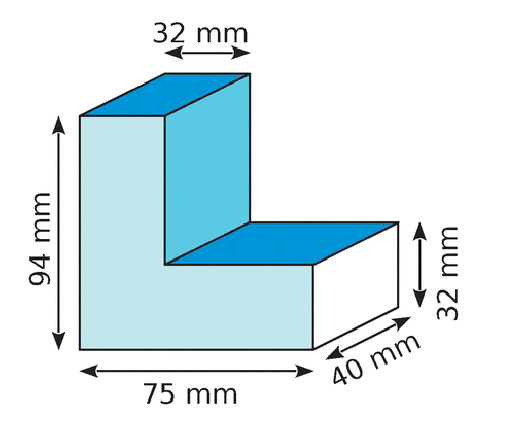
\includegraphics[scale=1]{vol2.eps} \\

Formule(s) utilisée(s) : . . . . . . . . . . . . . . . . . . .\\

Calculs :\\
\reponse[3]\\

Réponse : . . . . . . . . . . . . . . . . . . .\\

\exo \\ Calculer le volume du solide suivant. \\

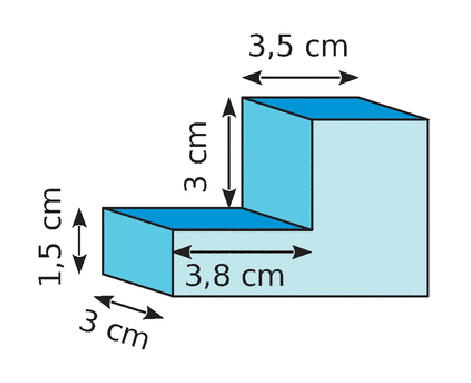
\includegraphics[scale=1]{vol3.eps} \\

Formule(s) utilisée(s) : . . . . . . . . . . . . . . . . . . .\\

Calculs :\\
\reponse[3]\\

Réponse : . . . . . . . . . . . . . . . . . . .\\

\exo \\ Calculer le volume du solide suivant. \\

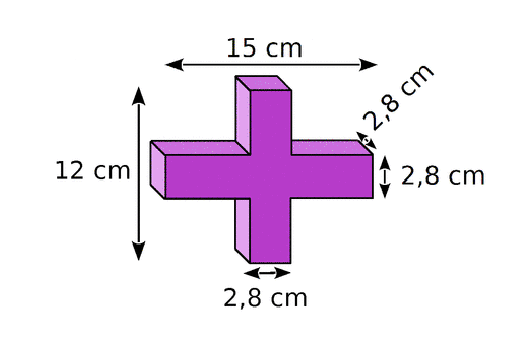
\includegraphics[scale=1]{vol4.eps} \\

Formule(s) utilisée(s) : . . . . . . . . . . . . . . . . . . .\\

Calculs :\\
\reponse[3]\\

Réponse : . . . . . . . . . . . . . . . . . . .\\











\begin{center}
{\Large \textbf{Niveau 5 :}}
\end{center}

\vspace*{1cm}

$\rightarrow$ \textbf{Vocabulaire (sommet, arête, face …)}\\

\vspace*{0.5cm}


\exo \\ On a marqué le cube ci-dessous en couleur sur le centre de quatre faces.\\

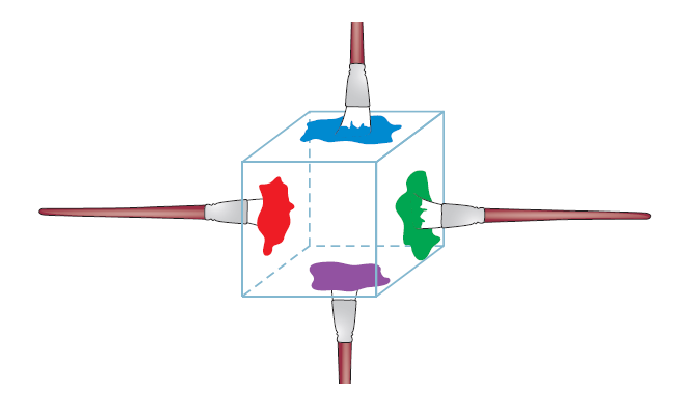
\includegraphics[scale=1]{voca8.eps} \\

Parmi les patrons suivants quels sont ceux qui correspondent au cube ci-dessus ?\\

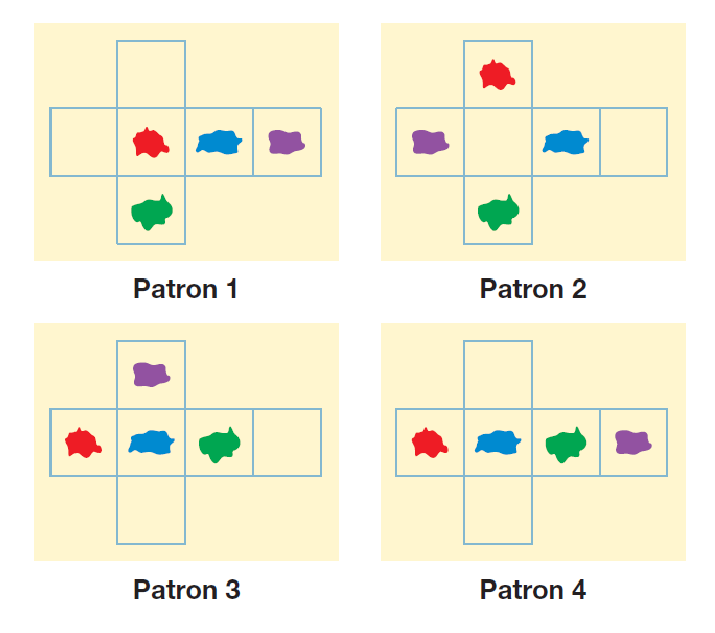
\includegraphics[scale=1]{voca9.eps} \\
\reponse[1]\\

\exo \\ Compléter le tableau ci-dessous à l'aide des figures suivantes.\\

\begin{flushleft}
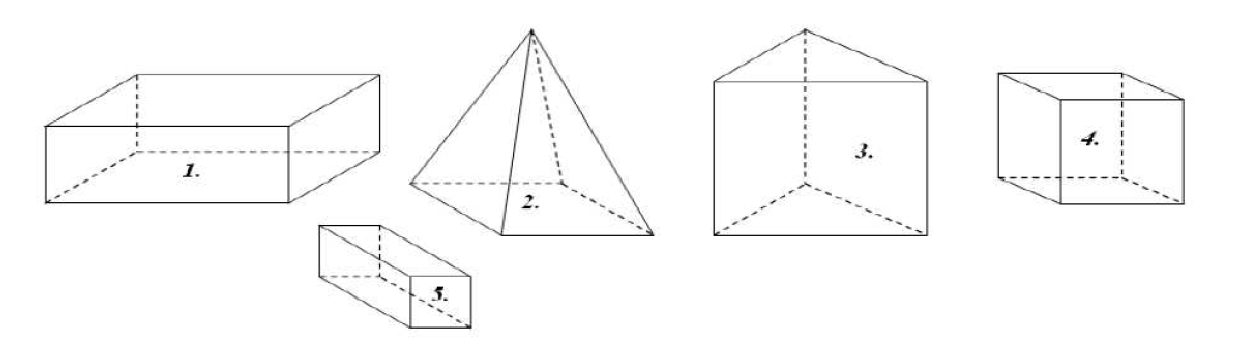
\includegraphics[scale=0.95]{voca10.eps} 
\end{flushleft}


\begin{tabular}{|c|c|c|c|c|c|}
\hline 
FIGURE & 1. & 2. & 3. & 4. & 5. \\ 
\hline 
Nombre de faces & . . . . & . . . . & . . . . & . . . . & . . . . \\ 
\hline 
Nombre d'arêtes & . . . . & . . . . & . . . . & . . . . & . . . . \\
\hline 
Nombre de sommets & . . . . & . . . . & . . . . & . . . . & . . . . \\
\hline 
Parallélépipède rectangle ? (oui/non) & . . . . & . . . . & . . . . & . . . . & . . . . \\
\hline 
\end{tabular} 

\vspace*{1cm}

$\rightarrow$ \textbf{Conversion de $m^{3}$}\\

\vspace*{0.5cm}





\exo \\ Convertir dans l'unité demandée.\\

\initqa \qa 43 000 $cm^{3}$ = . . . $dm^{3}$.\\

\qa 5,7 $m^{3}$ = . . . $dm^{3}$.\\


\qa 0,0026 $m^{3}$ = . . . $cm^{3}$.\\


\qa 500 L = . . . $m^{3}$.\\

\qa 720 $cm^{3}$ = . . . L.\\

\qa 31 mL = . . . $cm^{3}$.\\


\exo \\ Un litre d'eau pèse 1 kg. Combien pèse alors 15 $m^{3}$ d'eau?\\

Calculs :\\
\reponse[2]\\


Réponse : . . . . . . . . . . . . . . . . . . . . .\\



\exo \\ Un litre d'eau pèse 1 kg. Combien pèse alors 3 $cm^{3}$ d'eau?\\

Calculs :\\
\reponse[2]\\


Réponse : . . . . . . . . . . . . . . . . . . . . .\\



\exo \\ Un litre d'eau pèse 1 kg. Combien pèse alors 35 hL d'eau?\\

Calculs :\\
\reponse[2]\\


Réponse : . . . . . . . . . . . . . . . . . . . . .\\



\exo \\ Compléter avec la bonne unité ou la bonne conversion.\\

\initqa \qa 131,5 L = . . . . . . $m^{3}$\\

\qa 98,032 $cm^{3}$ = . . . . . . dL\\

\qa 4 103 L = 0,004 103  . . . . \\

\qa 100 000 000 $mm^{3}$ = 100 . . . .\\











\vspace*{1cm}

$\rightarrow$ \textbf{Calcul de volume}\\

\vspace*{0.5cm}



\exo \\ Mélanie a réalisé l'empilement ci-dessous.\\

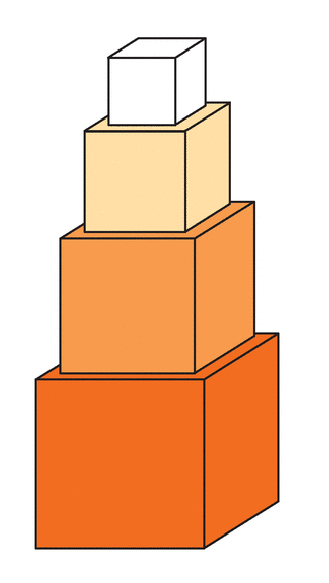
\includegraphics[scale=1]{vol5.eps} \\

Calculer son volume sachant que le côté du plus gros cube mesure 10 cm et que les côtés des autres cubes mesurent 2 cm de moins que celui du dessous.\\

Formule(s) utilisée(s) : . . . . . . . . . . . . . . . . . . .\\

Calculs :\\
\reponse[3]\\

Réponse : . . . . . . . . . . . . . . . . . . .\\


\exo \\ Comparer les figures ci-dessous et trouver celle qui a le plus grand volume.\\

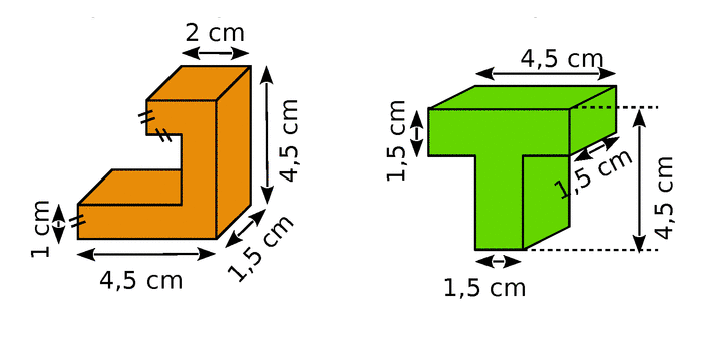
\includegraphics[scale=1]{vol6.eps} \\

Formule(s) utilisée(s) : . . . . . . . . . . . . . . . . . . .\\

Calculs :\\
\reponse[3]\\

Réponse : . . . . . . . . . . . . . . . . . . .\\


\exo \\ Un bac à fleurs est réalisé en bois à l'aide de planche de 12 mm d'épaisseur.\\
La longueur du bac est de 110 cm, sa largeur de 65 cm et sa hauteur de 45 cm (ces dimensions sont mesurées à l'extérieur).\\


Combien de sac de terre de 25 L faut-il acheter pour remplir le bac ?\\

Calculs :\\
\reponse[3]\\

Réponse : . . . . . . . . . . . . . . . . . . .\\








\end{document}
